\section{Spieler-Interface}

% Aus dem Wiki
% ------------
%
% Siehe: https://sopra.informatik.uni-freiburg.de/soprawiki/index.php?title=GDD#Spieler-Interface
%
% Dieser Abschnitt beinhaltet eine Beschreibung des Spielbildschirms, also
% dessen, was für den Spieler sichtbar ist. Dies beinhaltet die Art der
% Darstellung (2D oder 3D), die Kamerasicht, usw.
%
% Wichtig ist, dass alle sichtbaren Elemente, wie Minimap, Menüleiste, etc.
% erklärt werden. Durch ein Bild eines typischen Vertreters dieser Spielart
% oder durch eine Konzeptzeichnung des Interfaces kann die Beschreibung noch
% verbessert werden. In der finalen Version des GDDs können auch Screenshots
% des eigenen Spiels verwendet werden.
%
% Außerdem wird in diesem Abschnitt erklärt, wie der Spieler das Spiel steuert
% (mit der Maus, mit Maus und Tastatur, Joystick, Gamepad usw.). Alle Aktionen,
% die der Spieler durchführen kann, müssen erklärt werden. Auch mögliche
% Shortcuts und/oder Tastenkombinationen sollten hier erwähnt werden.
%
%
% Aus den Folien
% --------------
%
% Siehe: https://sopra.informatik.uni-freiburg.de/soprawiki/images/1/11/How-To-GDD_SS19.pdf
%
% * Beschreibung dessen, was der Spieler sieht
% * Art der Darstellung, Kameraansichten, sichtbare Elemente (HUD, Minimap,
%   Menüleisten, usw.)
% * Bild (Konzeptzeichnung, Screenshot, Mockup) dessen, wie das Spiel aussehen
%   soll.
% * Beschreibung der Steuerung.

\missingSection{spieler-interface}
Abbildung \ref{fig:spieler-interface} zeigt eine typische Momentaufnahme des Spiels \textit{Kernel Panic!}.
Der Spieler betrachtet die Spielwelt aus der Top-Down Perpektive.\\
Beschreiben wir zunächst das Head-up-Display (HUD) bestehend aus den rot markierten Bereichen mit den Nummerierungen $1$ bis $6$:
\begin{itemize}
	\item{1 Spielstand} Hier werden die wichtigsten Informationen angezeigt um direkt einen Überblick ins Spiel zu bekommen, vergleichbar mit einem Punktestand.
		\subitem{1 A:} Die aktuelle \textit{Spielzeit} zeigt an wielange das Spiel schon dauert.
		\subitem{1 B:} Direkt unter der \textit{Spielzeit} sind die erfolgreich Besiegten \textit{Wellen} im Überblick zu sehen. Links die Eigenen, rechts die des Gegners.
		\subitem{1 $C_{1}$ \& $C_{2}$:} $C_{1}$ zeigt die \textit{Erfahrungspunkte}, die man sich erspielt hat, $C{2}$ die des Gegners.
		\subitem{$D_{1}$ \& $D_{2}$:} Die aktuelle Ladung der Spieler. Hier gilt ebenfalls, links die eigenen auf der rechten Seite die des Gegners.
	\item {2 Verteidigungsgebäude} Oben am linken Bildrand ist eine Liste an \textit{Verteidigungsgebäuden}. Um zwischen den verschiedenen Gebäuden auszuwählen kann man die Tafeln 2 A bis 2 E benutzen.
	\item {3 \& 4 Angriffseinheiten:} Auf der gegenüberliegenden Seite des Bildschirms befinden sich die \textit{Angriffseinheiten}. Dabei sind 3 die \textit{Truppen }und 4 die \textit{Helden}. Auch hier kann man mit den verschiedenen Tafeln (3 A bis 3 E bzw 4 A bis 4 C) die genaue Auswahl treffen.
	\item {5 }
		\subitem{5 A:} \textit{Die Mini-map}
		\subitem{5 A:} Pause
		\subitem{5 A:} aktueller Kameraausschnitt markiert auf der Mini-map
	\item {6 Managment-Tafel:} Zeigt Info zu aktuell ausgewählt 
		\subitem{6 A bis C:} Aktionen des ausgewählt
		\subitem{6 D:} Bild des ausgewählt
		\subitem{6 E:} Status des ausgewählt
	\item {7 Mauszeiger} 
	\item {8 Mauszeigerturm}
	\item {9 CD Werfer der gerade feuert}
	\item {10 Mauszeigergeschoss}
	\item {11 Kabel}
	\item {12 Bug}
\end{itemize}
\begin{figure}[ht]
	\centering
	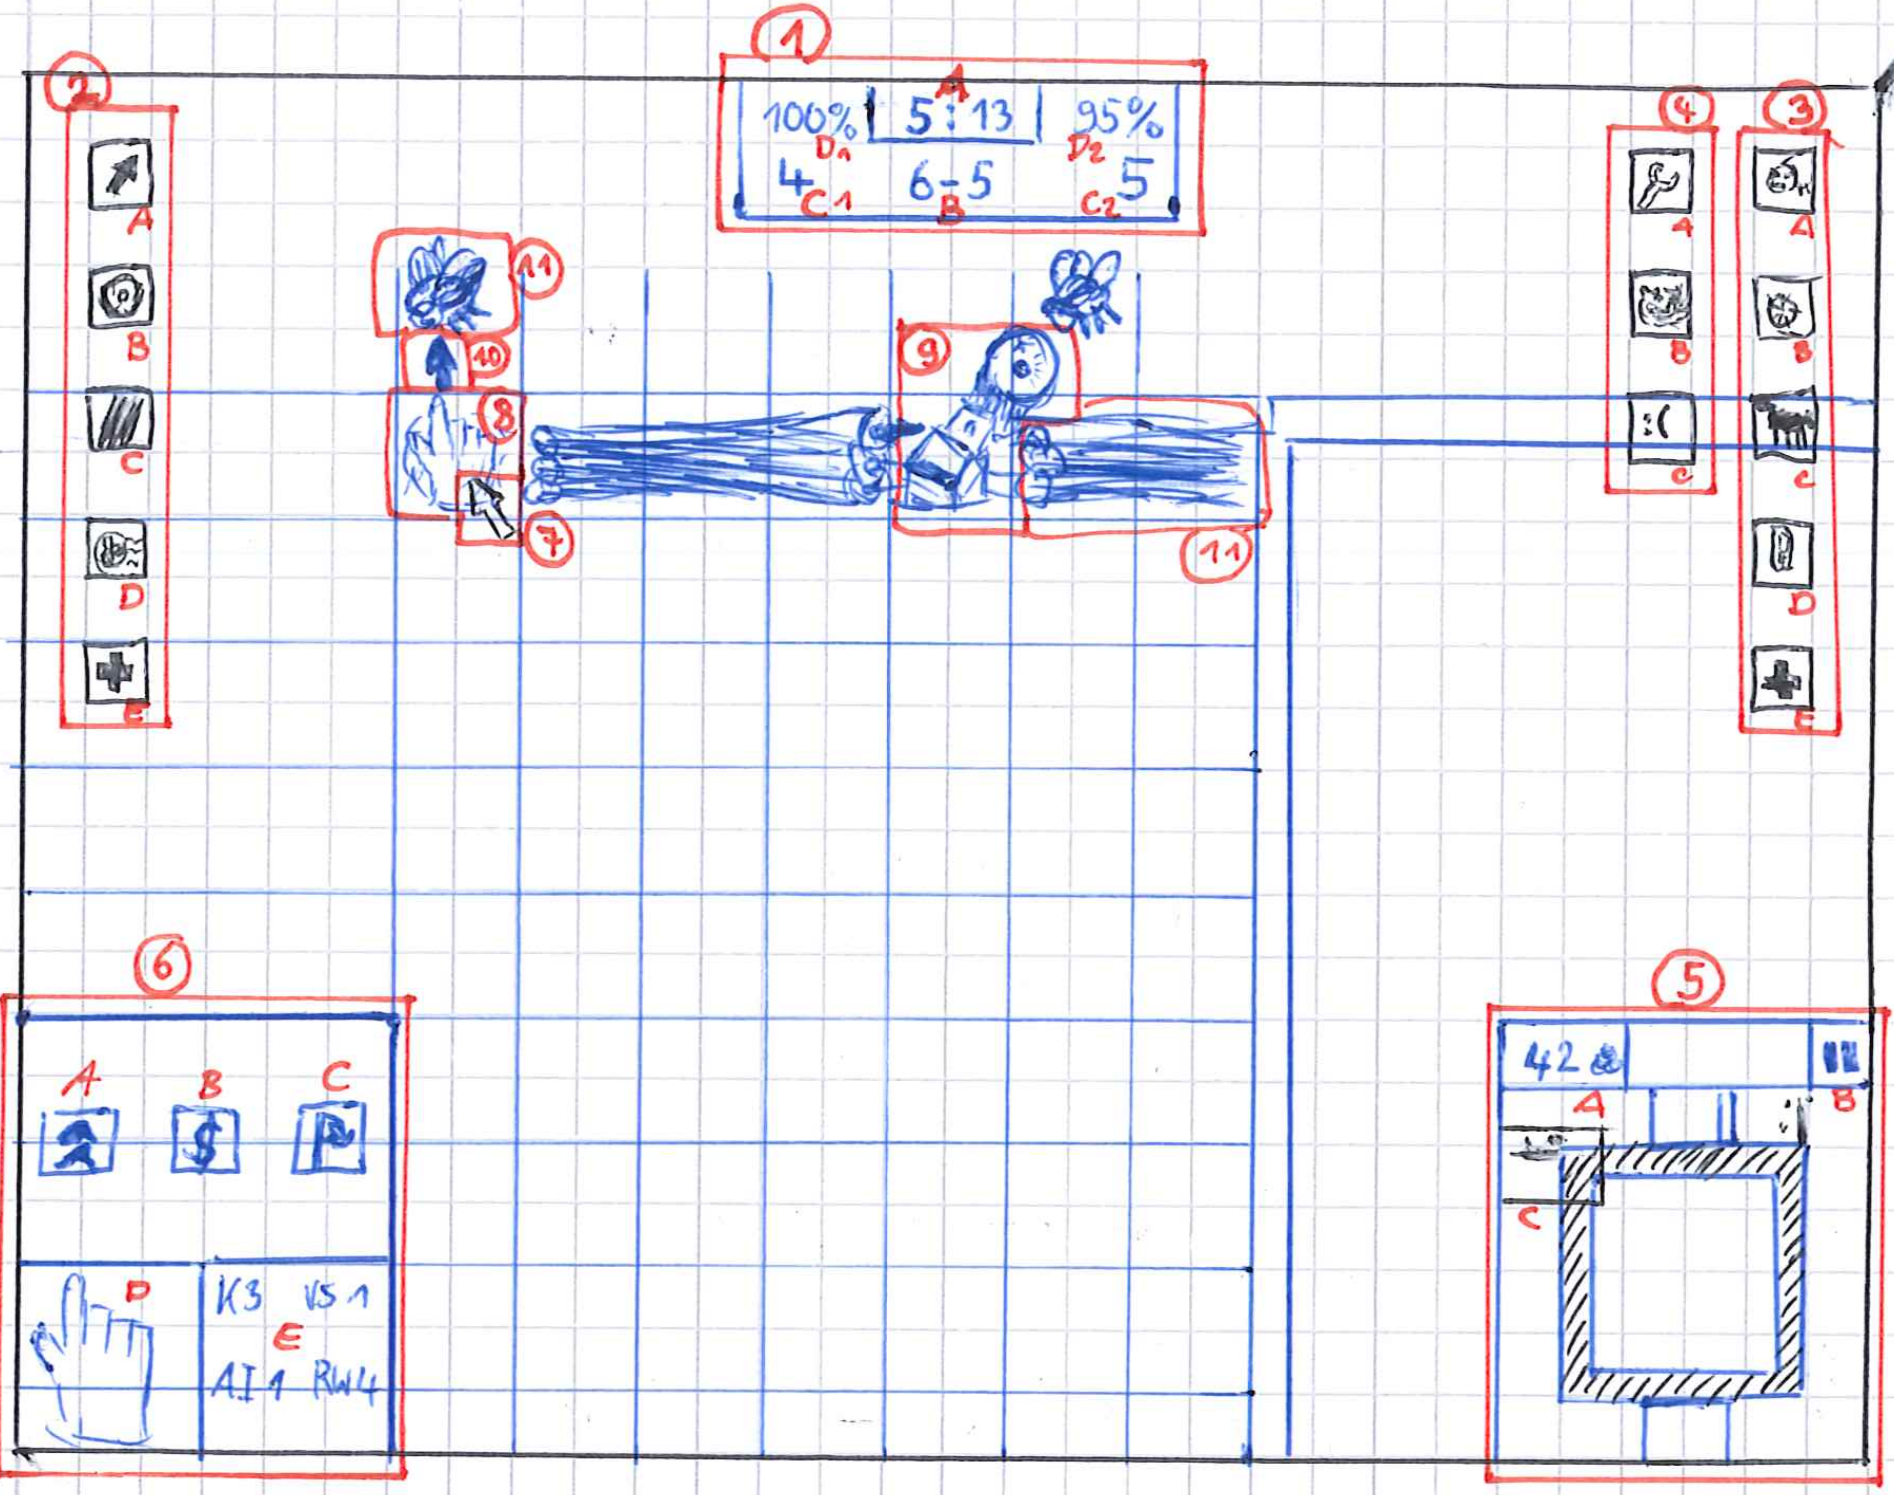
\includegraphics[width=1\textwidth]{spieler-interface.png}
	\caption{Spieler-Interface}
	\label{fig:spieler-interface}
\end{figure}
